\documentclass[tikz]{standalone}

\def\range{9}
\def\xyRatio{2/3}
\def\circSize{1mm}

\begin{document}
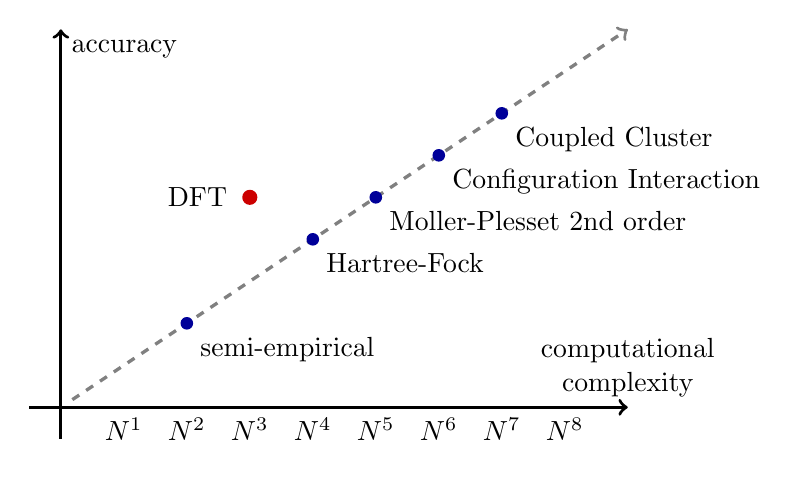
\begin{tikzpicture}[->, very thick, align=center, scale=0.8]

  \draw (0,-0.5) -- (0,\range*\xyRatio) node[below right] {accuracy};
  \draw (-0.5,0) -- (\range,0) node[above] {computational\\complexity};
  \foreach \n in {1,...,8}
  \node[below] at (\n,0) {$N^\n$};

  \draw[dashed, gray, shorten <=5] (0,0) -- (\range,\range*\xyRatio);

  \foreach \n/\name/\abbr in {2/semi-empirical/SE, 4/Hartree-Fock/HF, 5/Moller-Plesset 2nd order/MP2, 6/Configuration Interaction/CISD, 7/Coupled Cluster/CCSD(T)}
  \fill[blue!60!black] (\n,\xyRatio*\n) circle (\circSize)
  node[align=left, below right=1pt, black] (\abbr) {\name};

  % \draw[red, thick] (HF) -- (SE);

  \fill[red!80!black] (3,5*\xyRatio) circle (1.2*\circSize) node[left=1ex, black] {DFT};
  % \fill[blue!60!black] (4.5,6.5*\xyRatio) circle (\circSize) node[left=1ex, black] {Deep QMC};

\end{tikzpicture}
\end{document}
